% !TeX program = pdfLaTeX
\documentclass[12pt]{article}
\usepackage{amsmath}
\usepackage{graphicx,psfrag,epsf}
\usepackage{enumerate}
\usepackage{natbib}
\usepackage{textcomp}
\usepackage[hyphens]{url} % not crucial - just used below for the URL
\usepackage{hyperref}
\providecommand{\tightlist}{%
  \setlength{\itemsep}{0pt}\setlength{\parskip}{0pt}}

%\pdfminorversion=4
% NOTE: To produce blinded version, replace "0" with "1" below.
\newcommand{\blind}{0}

% DON'T change margins - should be 1 inch all around.
\addtolength{\oddsidemargin}{-.5in}%
\addtolength{\evensidemargin}{-.5in}%
\addtolength{\textwidth}{1in}%
\addtolength{\textheight}{1.3in}%
\addtolength{\topmargin}{-.8in}%

%% load any required packages here


\usepackage{color}
\usepackage{fancyvrb}
\newcommand{\VerbBar}{|}
\newcommand{\VERB}{\Verb[commandchars=\\\{\}]}
\DefineVerbatimEnvironment{Highlighting}{Verbatim}{commandchars=\\\{\}}
% Add ',fontsize=\small' for more characters per line
\usepackage{framed}
\definecolor{shadecolor}{RGB}{248,248,248}
\newenvironment{Shaded}{\begin{snugshade}}{\end{snugshade}}
\newcommand{\AlertTok}[1]{\textcolor[rgb]{0.94,0.16,0.16}{#1}}
\newcommand{\AnnotationTok}[1]{\textcolor[rgb]{0.56,0.35,0.01}{\textbf{\textit{#1}}}}
\newcommand{\AttributeTok}[1]{\textcolor[rgb]{0.77,0.63,0.00}{#1}}
\newcommand{\BaseNTok}[1]{\textcolor[rgb]{0.00,0.00,0.81}{#1}}
\newcommand{\BuiltInTok}[1]{#1}
\newcommand{\CharTok}[1]{\textcolor[rgb]{0.31,0.60,0.02}{#1}}
\newcommand{\CommentTok}[1]{\textcolor[rgb]{0.56,0.35,0.01}{\textit{#1}}}
\newcommand{\CommentVarTok}[1]{\textcolor[rgb]{0.56,0.35,0.01}{\textbf{\textit{#1}}}}
\newcommand{\ConstantTok}[1]{\textcolor[rgb]{0.00,0.00,0.00}{#1}}
\newcommand{\ControlFlowTok}[1]{\textcolor[rgb]{0.13,0.29,0.53}{\textbf{#1}}}
\newcommand{\DataTypeTok}[1]{\textcolor[rgb]{0.13,0.29,0.53}{#1}}
\newcommand{\DecValTok}[1]{\textcolor[rgb]{0.00,0.00,0.81}{#1}}
\newcommand{\DocumentationTok}[1]{\textcolor[rgb]{0.56,0.35,0.01}{\textbf{\textit{#1}}}}
\newcommand{\ErrorTok}[1]{\textcolor[rgb]{0.64,0.00,0.00}{\textbf{#1}}}
\newcommand{\ExtensionTok}[1]{#1}
\newcommand{\FloatTok}[1]{\textcolor[rgb]{0.00,0.00,0.81}{#1}}
\newcommand{\FunctionTok}[1]{\textcolor[rgb]{0.00,0.00,0.00}{#1}}
\newcommand{\ImportTok}[1]{#1}
\newcommand{\InformationTok}[1]{\textcolor[rgb]{0.56,0.35,0.01}{\textbf{\textit{#1}}}}
\newcommand{\KeywordTok}[1]{\textcolor[rgb]{0.13,0.29,0.53}{\textbf{#1}}}
\newcommand{\NormalTok}[1]{#1}
\newcommand{\OperatorTok}[1]{\textcolor[rgb]{0.81,0.36,0.00}{\textbf{#1}}}
\newcommand{\OtherTok}[1]{\textcolor[rgb]{0.56,0.35,0.01}{#1}}
\newcommand{\PreprocessorTok}[1]{\textcolor[rgb]{0.56,0.35,0.01}{\textit{#1}}}
\newcommand{\RegionMarkerTok}[1]{#1}
\newcommand{\SpecialCharTok}[1]{\textcolor[rgb]{0.00,0.00,0.00}{#1}}
\newcommand{\SpecialStringTok}[1]{\textcolor[rgb]{0.31,0.60,0.02}{#1}}
\newcommand{\StringTok}[1]{\textcolor[rgb]{0.31,0.60,0.02}{#1}}
\newcommand{\VariableTok}[1]{\textcolor[rgb]{0.00,0.00,0.00}{#1}}
\newcommand{\VerbatimStringTok}[1]{\textcolor[rgb]{0.31,0.60,0.02}{#1}}
\newcommand{\WarningTok}[1]{\textcolor[rgb]{0.56,0.35,0.01}{\textbf{\textit{#1}}}}


\usepackage{booktabs}
\usepackage{longtable}
\usepackage{array}
\usepackage{multirow}
\usepackage{wrapfig}
\usepackage{float}
\usepackage{colortbl}
\usepackage{pdflscape}
\usepackage{tabu}
\usepackage{threeparttable}
\usepackage{threeparttablex}
\usepackage[normalem]{ulem}
\usepackage{makecell}

\begin{document}


\def\spacingset#1{\renewcommand{\baselinestretch}%
{#1}\small\normalsize} \spacingset{1}


%%%%%%%%%%%%%%%%%%%%%%%%%%%%%%%%%%%%%%%%%%%%%%%%%%%%%%%%%%%%%%%%%%%%%%%%%%%%%%

\if0\blind
{
  \title{\bf Hyperparameter Tuning Strategies and Applications to Random
Forests}

  \author{
        sr4376 \thanks{Thank you to Nick Horton for his help and
guidance in the creation of this project.} \\
    Department of Mathematics and Statistics, Amherst College\\
      }
  \maketitle
} \fi

\if1\blind
{
  \bigskip
  \bigskip
  \bigskip
  \begin{center}
    {\LARGE\bf Hyperparameter Tuning Strategies and Applications to
Random Forests}
  \end{center}
  \medskip
} \fi

\bigskip
\begin{abstract}
The text of your abstract. 200 or fewer words. Hyperparameter tuning has
recently emerged within the field of machine learning as a popular
method to determine the most optimal combination of hyperparameters to
maximize model performance. As a meta-learning problem, several popular
approaches such as grid search, random search, and sequential
model-based optimization methods have been proposed to achieve this. In
this report, we explore, implement, and explain how these these methods
work. We also perform some application studies to classification
problems with certain datasets in order to compare and contrast their
effectiveness and runtimes, alongside performing a case-study on
language learning abilities using our findings.
\end{abstract}

\noindent%
{\it Keywords:} machine learning, classification, meta learning, model
parameter, hyperparameter
\vfill

\newpage
\spacingset{1.45} % DON'T change the spacing!

\hypertarget{introduction}{%
\section{Introduction}\label{introduction}}

\label{sec:intro}

Machine Learning is a rapidly evolving subfield of artificial
intelligence widely utilized by practitioners in fields ranging from
health care, sciences, government, and many more disciplines because of
its practicality and usefulness especially in these times where data is
more accessible and prevalent than ever. As its name suggests, many of
the techniques in machine learning have to do with the training of a
computer (machine) to learn from data and use it to execute a program to
solve a problem at hand.

These problems can range from simple tasks such as trying to generate a
``rule'' to differentiate between groups such as apples and oranges
(classification task), trying to find unknown clusters in a set of data
(clustering), etc. It would be difficult to go into the details and
specifics within the types of learning that machine learning
encompasses, as there are far too many machine learning tasks to cover
in a single report -- but the most important takeaway would have to be
the ability of machine learning algorithms to develop, learn, and train
from data to create models.

While in the process of creating these models, it can often be
challenging to find the model which best captures the information from
the training data. Depending on what sort of machine learning task is in
question (classification, clustering, reinforcement learning, etc.) each
model takes in unique parameters known as `hyperparameters,' which
govern the training process itself.

For example, if we were looking at clustering as a technique
(specifically K-Means clustering) -- some hyperparameters to alter would
be things such as: the number of clusters we want, the initial
configuration of centroids, the max number of iterations we want the
algorithm to run, etc. Altering these hyperparameters (aka.
model-specific properties) can often change how the model fits and
adheres to the training data. Thus, it is important to choose
hyperparameters that allows for the model to best adapt to the training
data without underfitting or overfitting to the data.

How do we pick the correct configuration of parameters to use then? The
process of creating these models itself is a sub-field known as
``meta-learning,'' and many techniques have been founded and developed
to tackle the challenges of finding the best model for a given task. One
of the most notable methods of meta-learning tasks is known as
``hyperparameter tuning,'' which will be the focus of this report.

Hyperparameter tuning is essentialy an optimization task, in which we
are trying to look for the best combinations of hyperparameters to use
to train our model. Methods such as grid search, random search, and
Bayesian searches have come up in recent times which aid machine
scientists to obtain the set of hyperparameters which builds the best
performing model.

\newpage

\hypertarget{background}{%
\section{Background}\label{background}}

\label{sec:background}

\hypertarget{model-parameters-and-hyperparameters}{%
\subsection{Model Parameters and
Hyperparameters}\label{model-parameters-and-hyperparameters}}

\label{sec:param_hyperparam}

An important conceptualization of a model parameter and hyperparameter
is essential to understanding the underpinnings of model tuning and
meta-learning. These are terms which are often confused for one another
in machine learning. A \emph{model parameter}, in terms of machine
learning algorithms, is a variable whose value is estimated from the
dataset, NOT by the user. For example, the coefficients/effects of the
explanatory variables in a linear regression model are known as model
parameters. Some other model parameters in machine learning include
weights and biases which are important to the functioning of in neural
networks \citep{Yang2020}.

A hyperparameter on the other hand is a variable whose value is set by
the user before the model training begins. These values can freely be
adjusted by the user in order to obtain different models, and as such,
it is important to set model parameters correctly in order to obtain
models with optimal performance. An example of a model hyperparameter
can be variables such as \(k\) (the number of clusters) in a clustering
algorithm.

Misspecification of model hyperparameters are detrimental to machine
learning models' performance. If we think about clustering as a
technique we wish to run in order to differentiate between different
types of fruit (say, apples and oranges), and the user specified an
unreasonable number of clusters \(k\) such as 100, the model clearly
would not be able to find the correct clusters in the data due to
misspecification of the number of clusters \(k\). The model would
perform at a much more reasonable level if the user had instead
specified a \(k\) of 2.

However, how would the user know what values are the most optimal to
pick in order to achieve the most optimum level? This is where
hyperparameter tuning can assist us.

\hypertarget{hyperparameter-tuning}{%
\subsection{Hyperparameter Tuning}\label{hyperparameter-tuning}}

\label{sec:tuning}

Hyperparameter tuning works in a variety of ways but it generally
involves running an algorithm in order to find the combination of
optimum combinations of hyperparameters and the methods to do have are
varied and differ in their approaches. The core of all tuning algorithms
involves running multiple trials with a variety of combinations of
hyperparameters and identifying which combination minimizes (or
maximizes) the loss function metric the user specifies (accuracy,
misclassification rate, etc.).

To get a better sense of things (i.e, why hyperparameter tuning is
important/helpful), the following section will discuss how
hyperparameter tuning with regards to classification trees. In
classification, our goal is of course, to create a model which is able
to predict which class a certain observation belongs to. An example
classification task will be performed with the \texttt{palmerpenguins}
dataset which contains observations regarding body measurements and
other supplementary information for 344 penguins collected from the
Palmer Archipelago. The classification task at hand will be to create a
classification tree model which is able to predict the \texttt{species}
from the following ``Adelie,'' ``Gentoo,'' and ``Chinstrap'' penguins
which comprise the dataset.

The difficulty in creating classification tree models which are
meaningful lies in the splitting and pruning the trees itself. First and
foremost, trees generally perform splits on variables in order to
differentiate between classes. For example in our
\texttt{palmerpenguins} dataset, we may want to create a split on the
variable \texttt{bill\_length\_mm} and claim that a
\texttt{bill\_length\_mm} of \textless{} 40 usually means that the
penguin is an ``Adelie'' penguin, and those with
\texttt{bill\_length\_mm} \textgreater= 40 usually are ``Gentoo'' and
``Chinstrap'' penguins. In general, splits in which the groups are
mostly pure are the most ideal -- if a node is 100\% pure, it means that
all observations in that node belong to the same class.

In creating a classification tree model, it is possible to specify
\texttt{minsplit}, the minimum number of observations which must exist
in a node in order for a split to be attempted, \texttt{minbucket}, the
minimum number of observations in any terminal/leaf node, etc. These are
the hyperparameters for creating a decision tree.

We will create and feature two unique decision tree models for the
\texttt{palmerpenguins} data set using distinct combinations for
\texttt{minsplit} and \texttt{minbucket} to show how the model output
can vary with a slight tweak to these values.

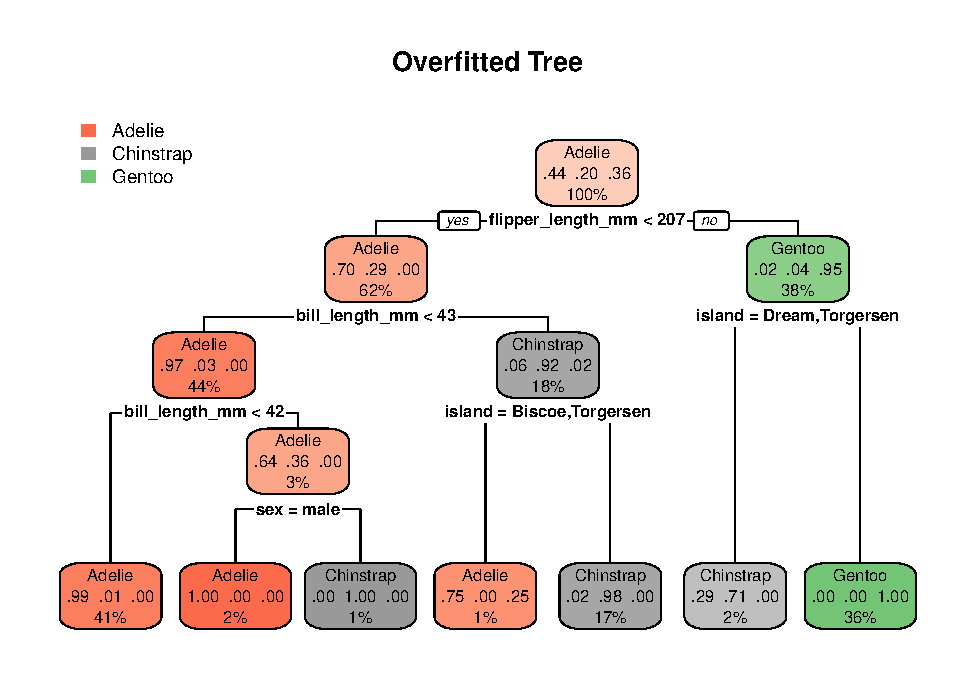
\includegraphics{deid_files/figure-latex/tree1.1-1.pdf}

The first classification tree created used a \texttt{minsplit} = 10 and
\texttt{minbucket} = 2. The following rules set by these hyperparameter
dictates the following: while creating the tree, the algorithm only
splits a node if it has more than 10 observations in it, and if a split
would create a new node with less than 2 observations. Due to the
\texttt{minsplit} value being rather small, the algorithm will be quite
liberal with splitting nodes (it keeps splitting nodes if they have more
than 10 observations), and also is quite generous with what sort of
nodes are being created (nodes of size 2 or larger are deemed fine to
make). This is obviously quite troublesome as the values that we set for
these hyperparameters yield which is rather descriptive and difficult to
interpret as it seems to overfit the data tremendously.

Altering the hyperparameters to have \texttt{minsplit} = 30, and
\texttt{minbucket} = 15, to obtain a new tree then, will yield:

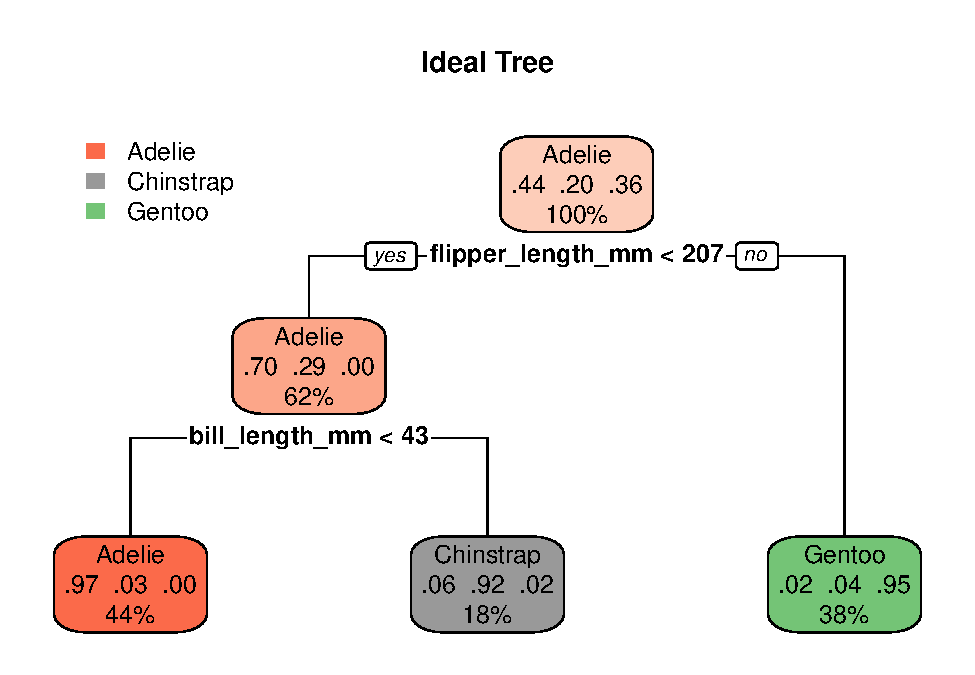
\includegraphics{deid_files/figure-latex/tree2.1-1.pdf}

In this tree, more reasonable values of \texttt{minsplit} and
\texttt{minbucket} are chosen, in which a split is considered if a node
has observatiosn \textgreater= 30, and if a split would make a node that
has less than 15 observations, it won't split the node. The second set
of hyperparameters yields a tree which isn't as overfit as seen in the
first tree, as a result of picking good hyperparameter values.

Thus from this in-depth study on classification trees and the
hyperparameters which dictate the algorithm's behavior in creating a
decision tree model, it can be seen that picking good hyperparamter
values is essential -- not just for decision tree model making, but all
types of machine learning models also. It can be quit troublesome to
determine what sorts of hyperparameter values to pick, and that fact
compounded by the myriad of machine learning techniques out there makes
it quite bothersome to have to go through multiple combinations of
hyperparameter values in a model just to see which one is the most
optimum, which is why hyperparameter optimization/tuning is essential.

A more in-depth discussion on how the hyperparameter methods perform and
work will be discussed in the methods section \ref{sec:methods}.

\newpage

\hypertarget{question}{%
\section{Question}\label{question}}

\label{sec:question}

The focus of my project specifically encompasses hyperparameter tuning
and optimization with regards to ensemble-learning algorithms --
specifically classification with random forests, and studying the
effectiveness of three different hyperparameter tuning techniques: grid
search, random search, and Bayesian hyperparameter optimization -- with
regards to large data. A further discussion on these methods will
follow.

\hypertarget{methods}{%
\section{Methods}\label{methods}}

\label{sec:methods}

Grid search (which will be implemented with the \texttt{caret} package
in R) is a brute-force/exhaustive algorithm where the user specifies a
list of values for hyperparameters and the computer evaluates the
performance of each combination, which allows us to observe the most
optimum combination of values. Although this method guarantees that the
most optimal configuration of hyperparameters will be found at the
search's conclusion, the issue lies in the runtime. As a brute force
approach whose runtime is dependent on the number of hyperparameters
given, we can expect the time-complexity of this approach to be quite
abysmal. Grid search has been found to be reliable in low dimensional
spaces however, and is simple to implement in cases when the
dimensionality of a dataset is low \citep{Bergstra2012}.

The idea of random search is quite similar to grid search, but instead
of evaluating each combination of hyperparameters like grid search does,
random search evaluates random combinations of a range hyperparameter
values until a criteria is met (like the maximum number of iterations
being reached). Random search will also be implemented using the
\texttt{caret} package in R. While random search sacrifices the
comprehensibility (looking every possible combination of
hyperparameters) of grid search, its runtime is far more feasible. Where
it falls short however is that due to the combinations being selected by
random chance, it can often yield high variance during computing.
Everything is being left to luck, which is quite risky
\citep{Bergstra2012}.

The most recent advances in hyperparameter tuning is Bayesian
hyperparameter optimization which as its name suggests, utilizes
Bayesian logic in order to select the most promising hyperparameters.
The specific type of Bayesian hyperparameter optimziation technique we
will be observing is the Sequential Model-based Optimization (with the
\texttt{tuneranger} package in R) which creates and evaluates models
based on previous iterations and chooses future combinations while
considering for these results. Essentially, with the line of Bayesian
reasoning, with more runs and combinations -- the model will eventually
become ``less wrong,'' and will settle on the best combination of
hyperparameters in fewer iterations that both grid search and random
search \citep{Probst2019}.

Sequential Model-Based Optimization essentially consists of the
following steps:

\begin{enumerate}
\def\labelenumi{\arabic{enumi})}
\item
  Specify an evaluation metric to use (RMSE, accuracy), evaluation
  strategy to test the model on (bagging, CV), and hyperparameters you
  wish to use in creating the model in question and create your initial
  model.
\item
  Based on the output from step 1, fit a regression model (aka.
  surrogate model) on all previously tested hyperparameters with the
  y-axis as the evaluation measure and hyperparameters as the x-axis
\item
  Based on the regression model in step 2, choose a new combination of
  hyperparameters with good performance metrics to create an updated
  model, evaluate the updated model, and then add it to the existing
  hyperparameter space.
\item
  Repeat steps 2-3 until a desired model is reached \citep{Probst2019}.
\end{enumerate}

The focus on the differences between these methods thus lie in their
runtimes. Each method will be able to find a combination of
hyperparameters which yield the most optimum model in accordance with
their principles, but the problem lies in how quickly these combinations
can be obtained alongside their ease of implementation and effectiveness
\citep{Probst2019}

\newpage

\hypertarget{example-cells}{%
\section{Example: Cells}\label{example-cells}}

\label{sec:cells}

To begin our investigation on the implementations of the tuning
algorithms, we will introduce \texttt{cells} a dataset which is featured
in the package \texttt{modeldata}, which contains information on cell
segmentation imaging -- with observations belonging to two classes
\texttt{WS}, well-segmented and \texttt{PS} poorly-segmented.

Each of the three aforementioned techniques will be implemented with
regards to creating a random forest classification model of the
\texttt{cells} dataset. A careful consideration of the runtimes and
effectiveness of each of the three methods will further be discussed as
well. In each implementation of the methods discussed, the length it
will take for the tuning algorithm to finish will be measured, to give a
sense of the feasbility of implementation of each respective method
towards a large-scale application to big data.

First, we will be implementing grid search as a means to find optimal
hyperparameters for our random forest.

\begin{verbatim}
## Random Forest 
## 
## 1414 samples
##   56 predictor
##    2 classes: 'PS', 'WS' 
## 
## No pre-processing
## Resampling: Cross-Validated (10 fold, repeated 3 times) 
## Summary of sample sizes: 1273, 1272, 1272, 1273, 1273, 1272, ... 
## Resampling results across tuning parameters:
## 
##   mtry  min.node.size  splitrule   Accuracy   Kappa    
##   2     1              gini        0.8210818  0.6046983
##   2     1              extratrees  0.8246312  0.6108339
##   2     2              gini        0.8201462  0.6025475
##   2     2              extratrees  0.8232111  0.6074868
##   2     3              gini        0.8206090  0.6041247
##   2     3              extratrees  0.8234542  0.6074702
##   2     4              gini        0.8217960  0.6057111
##   2     4              extratrees  0.8210885  0.6031265
##   2     5              gini        0.8196684  0.6015207
##   2     5              extratrees  0.8236889  0.6085264
##   3     1              gini        0.8180185  0.5991875
##   3     1              extratrees  0.8255752  0.6144244
##   3     2              gini        0.8196684  0.6030214
##   3     2              extratrees  0.8229714  0.6092367
##   3     3              gini        0.8189525  0.6013357
##   3     3              extratrees  0.8255719  0.6144392
##   3     4              gini        0.8192072  0.6019067
##   3     4              extratrees  0.8234609  0.6096309
##   3     5              gini        0.8189542  0.6010108
##   3     5              extratrees  0.8227450  0.6073612
##   4     1              gini        0.8189608  0.6018339
##   4     1              extratrees  0.8286452  0.6226389
##   4     2              gini        0.8159075  0.5949279
##   4     2              extratrees  0.8253371  0.6150530
##   4     3              gini        0.8189575  0.6017652
##   4     3              extratrees  0.8272201  0.6187203
##   4     4              gini        0.8227300  0.6096817
##   4     4              extratrees  0.8241684  0.6125730
##   4     5              gini        0.8201495  0.6040278
##   4     5              extratrees  0.8277012  0.6193033
##   5     1              gini        0.8203809  0.6051652
##   5     1              extratrees  0.8258016  0.6163377
##   5     2              gini        0.8184913  0.6023222
##   5     2              extratrees  0.8293510  0.6242140
##   5     3              gini        0.8163720  0.5963900
##   5     3              extratrees  0.8246379  0.6133476
##   5     4              gini        0.8161389  0.5961443
##   5     4              extratrees  0.8269820  0.6179442
##   5     5              gini        0.8208504  0.6062000
##   5     5              extratrees  0.8260430  0.6171596
## 
## Accuracy was used to select the optimal model using the largest value.
## The final values used for the model were mtry = 5, splitrule = extratrees
##  and min.node.size = 2.
\end{verbatim}

\begin{verbatim}
## Time difference of 3.530586 mins
\end{verbatim}

Our grid search tuning algorithm took around 3 minutes to run, and it
suggested the following hyperparameters to use in order to achieve the
most optimal model (with accuracy and kappa metrics: mtry = 5, splitrule
= extratrees and min.node.size = 3. Although it is known that the
algorithm went over every possible combination of hyperparameters, and
thus, this is indeed most likely the best one, the amount of time this
method took is a bit concerning. In this example of grid search, the
tuning algorithm was offered 4 possible values for \texttt{mtry}, 5 for
\texttt{min.node.size}, and 2 for \texttt{splitrule}, leading to a total
of 4 \(*\) 5 \(*\) 2 \(=\) 40 different models to create. The more
hyperparameters one has to tune, the higher the runtime it will take
which is an important consideration to take into account.

\begin{verbatim}
## Random Forest 
## 
## 1414 samples
##   56 predictor
##    2 classes: 'PS', 'WS' 
## 
## No pre-processing
## Resampling: Cross-Validated (10 fold, repeated 3 times) 
## Summary of sample sizes: 1273, 1272, 1272, 1273, 1273, 1272, ... 
## Resampling results across tuning parameters:
## 
##   min.node.size  mtry  splitrule   Accuracy   Kappa    
##    2             52    extratrees  0.8199131  0.6051201
##    3             13    gini        0.8187294  0.6029201
##   14             51    extratrees  0.8229764  0.6108343
##   15             28    extratrees  0.8234442  0.6118789
##   17             29    gini        0.8145024  0.5940334
## 
## Accuracy was used to select the optimal model using the largest value.
## The final values used for the model were mtry = 28, splitrule = extratrees
##  and min.node.size = 15.
\end{verbatim}

\begin{verbatim}
## Time difference of 1.613703 mins
\end{verbatim}

Our random search tuning algorithm took around 1.27 minutes to run,
which is a marked improvement over the grid search implementation. The
output from this code suggested to pick the following values to obtain
the highest accuracy: mtry = 28, splitrule = extratrees and
min.node.size = 15. This method uses a small search space which is why
it runs much faster than the previous grid search. However, it is
important to note that random search yields high variance during
computing due to its `random' nature, and as such it may not also find
the most optimal configuration of hyperparameters as it leaves it up to
chance.

\begin{verbatim}
## Time difference of 1.743826 mins
\end{verbatim}

An alternative technique is to use \texttt{tuneRanger} which is a
specialized package in R useful for automatic tuning of random forests.
The tuning strategy used in \texttt{tuneRanger} is of a sequential
model-based optimization which essential iterates between fitted models
and uses past model fits as knowledge in the creation of new ones --
akin to Bayesian methods in statistics. This run took around 1.5 minutes
to run which is still a marked improvement over grid search and takes
only slightly longer than random search (the output obtained from
running SMBO is omitted due to its excessive length).

From the tuning algorithms, it can clearly be seen that even with the
rather small size of the \texttt{cells} dataset -- the hyperparameter
tuning algorithms took a considerably long time to run. This will be
important to note during the application of such methods on a
large-scale real-world dataset.

\newpage

\hypertarget{real-world-example}{%
\section{Real-World Example}\label{real-world-example}}

\label{sec:realworld}

Using knowledge gained from the previous section where we investigated
the effectiveness and capabilities of each of the three tuning methods,
we will begin a deep-dive into a large scale investigation on real-world
data, specifically investing the language learning capabilities of
individuals.

There is a commonly known belief that children learn languages much
better than adults, but there is a lack of empirical evidence to support
this which is why several researchers have conducted a large study with
over 600,000 English learners (with participants from all facets of
life) and conducted an English grammar test for all participants to
assess these beliefs. Information in the dataset consist of demographic
variables of the study partcipants alongside the proportion of correct
answers in their grammar test.

We will be creating a ML classification task, specifically a random
forest model, to aid in identifying individuals based on their skill
levels (which we will assume to be connected directly to their English
grammar test). Individuals are grouped into 4 distinct groups based on
the proportion of answers the got correct on their test: ``\textless{}
0.85'', ``0.850-0.899'', ``0.900-0.949'', and ``\textgreater{} 0.95''.

Grid search and random search will not be implemented in this analysis
as it simply takes up too much computational time and is unfeasible to
utilize with the scale of our data (left machine to run grid search and
random search on language learning data, and it took over a day/24
hours, and it still did not complete). As a result of this, model tuning
will be handled with SMBO.

Omitting grid search and random search, and running SMBO directly:

The SMBO method took 48.72681 minutes to complete. From the output, it
is suggested to use the following hyperparameters: \texttt{mtry} = 20,
\texttt{min.node.size} = 3558, and \texttt{sample.fraction} = 0.5818905,
which yields a Brier score of 0.

\newpage

Creating this model then:

\begin{verbatim}
##              
##               < 0.85 0.850-0.899 0.900-0.949 > 0.95
##   < 0.85       10749           0           0      0
##   0.850-0.899      0       10967           0      0
##   0.900-0.949      0           0       21458      0
##   > 0.95           0           0           0  20400
\end{verbatim}

Running the model with the suggested hyperparameters on the testing set,
a confusion matrix is obtained. We can see that every single observation
seems to be correctly classified.

Just to be sure that these optimum hyperparameters are just that,
optimum -- I created another random forest without some arbitrary
hyperparameters I personally picked:

\begin{verbatim}
##              
##               < 0.85 0.850-0.899 0.900-0.949 > 0.95
##   < 0.85       10492         118         137      2
##   0.850-0.899     29       10833          98      7
##   0.900-0.949      0           0       21458      0
##   > 0.95           0           0           0  20400
\end{verbatim}

We can see that there are far more incorrectly classified observations
this time for each skill group\ldots{}

It seems that in this example, hyperparameter tuning was not essential
to the creation of an accurate model, but the importance and function
that tuning algorithms provide, is not to be overlooked.

\newpage

\hypertarget{conclusion}{%
\section{Conclusion}\label{conclusion}}

\label{sec:conclusion}

Hyperparameter tuning is still a field which needs to be delved into
more and has the potential to be improved upon. Although helpful in
creating optimum ML models for any sort of ML-related task, we explored
in this project applications of tuning algorithms ranging from grid
search, random search, and sequential model-based optimization
techniques as well, each with their own distinct advantages and
downsides. Although helpful in certain cases when accuracy and
misclassification rates is of utmost importance, it is important to
consider whether or not if hyperparameter tuning is worth running for a
specific task. The amount of time that it takes to optimize a model with
tuning algorithms might not be worth the small amounts of improvements
that the most optimum hyperparameters may give it.

\newpage

\hypertarget{appendix}{%
\section{Appendix}\label{appendix}}

\label{sec:appendix}

\hypertarget{data}{%
\subsection{Data}\label{data}}

\begin{Shaded}
\begin{Highlighting}[]
\NormalTok{penguins <{-}}\StringTok{ }\NormalTok{palmerpenguins}\OperatorTok{::}\NormalTok{penguins}
\KeywordTok{library}\NormalTok{(modeldata)}
\KeywordTok{data}\NormalTok{(cells, }\DataTypeTok{package =} \StringTok{"modeldata"}\NormalTok{) }\CommentTok{\#cells data}

\NormalTok{cells <{-}}\StringTok{ }\NormalTok{cells }\OperatorTok{\%>\%}
\StringTok{  }\KeywordTok{select}\NormalTok{(}\KeywordTok{c}\NormalTok{(}\DecValTok{3}\OperatorTok{:}\DecValTok{58}\NormalTok{, }\DecValTok{2}\NormalTok{))}

\CommentTok{\#splitting training and testing}
\NormalTok{cells\_partition <{-}}\StringTok{ }\KeywordTok{createDataPartition}\NormalTok{(cells}\OperatorTok{$}\NormalTok{class, }
                                       \DataTypeTok{p =} \FloatTok{0.7}\NormalTok{, }\DataTypeTok{list =} \OtherTok{FALSE}\NormalTok{)}
\NormalTok{cells\_training <{-}}\StringTok{ }\NormalTok{cells[cells\_partition, ]}
\NormalTok{cells\_testing <{-}}\StringTok{ }\NormalTok{cells[}\OperatorTok{{-}}\NormalTok{cells\_partition, ]}

\CommentTok{\#defining variables and target}
\NormalTok{cells\_vars <{-}}\StringTok{ }\NormalTok{cells[,}\DecValTok{1}\OperatorTok{:}\DecValTok{56}\NormalTok{]}
\NormalTok{cells\_target <{-}}\StringTok{ }\NormalTok{cells[,}\DecValTok{57}\NormalTok{]}
\CommentTok{\#\# setting working directory}
\NormalTok{language <{-}}\StringTok{ }\KeywordTok{read\_csv}\NormalTok{(}\StringTok{"data/language\_learning\_cleaned.csv"}\NormalTok{)}

\NormalTok{language <{-}}\StringTok{ }\NormalTok{language }\OperatorTok{\%>\%}
\StringTok{  }\NormalTok{janitor}\OperatorTok{::}\KeywordTok{clean\_names}\NormalTok{() }\OperatorTok{\%>\%}
\StringTok{  }\KeywordTok{mutate}\NormalTok{(}\DataTypeTok{age\_group =} \KeywordTok{case\_when}\NormalTok{(}
\NormalTok{    age }\OperatorTok{<}\StringTok{ }\DecValTok{18} \OperatorTok{\textasciitilde{}}\StringTok{ "< 18"}\NormalTok{,}
\NormalTok{    age }\OperatorTok{>=}\StringTok{ }\DecValTok{18} \OperatorTok{\&}\StringTok{ }\NormalTok{age }\OperatorTok{<}\StringTok{ }\DecValTok{30} \OperatorTok{\textasciitilde{}}\StringTok{ "18{-}29"}\NormalTok{,}
\NormalTok{    age }\OperatorTok{>=}\StringTok{ }\DecValTok{30} \OperatorTok{\&}\StringTok{ }\NormalTok{age }\OperatorTok{<}\StringTok{ }\DecValTok{45} \OperatorTok{\textasciitilde{}}\StringTok{ "30{-}44"}\NormalTok{,}
\NormalTok{    age }\OperatorTok{>=}\StringTok{ }\DecValTok{45} \OperatorTok{\&}\StringTok{ }\NormalTok{age }\OperatorTok{<}\StringTok{ }\DecValTok{61} \OperatorTok{\textasciitilde{}}\StringTok{ "45{-}60"}\NormalTok{,}
\NormalTok{    age }\OperatorTok{>}\StringTok{ }\DecValTok{60} \OperatorTok{\textasciitilde{}}\StringTok{ "> 60"}\NormalTok{)) }\OperatorTok{\%>\%}
\StringTok{  }\KeywordTok{mutate}\NormalTok{(}\DataTypeTok{age\_group =} \KeywordTok{factor}\NormalTok{(age\_group, }
                            \DataTypeTok{levels =} \KeywordTok{c}\NormalTok{(}\StringTok{"< 18"}\NormalTok{, }\StringTok{"18{-}29"}\NormalTok{, }
                                       \StringTok{"30{-}44"}\NormalTok{, }\StringTok{"45{-}60"}\NormalTok{, }
                                       \StringTok{"> 60"}\NormalTok{))) }\OperatorTok{\%>\%}
\StringTok{  }\KeywordTok{mutate}\NormalTok{(}\DataTypeTok{skill\_group =} \KeywordTok{case\_when}\NormalTok{(}
\NormalTok{    correct }\OperatorTok{<}\StringTok{ }\FloatTok{0.85} \OperatorTok{\textasciitilde{}}\StringTok{ "< 0.85"}\NormalTok{,}
\NormalTok{    correct }\OperatorTok{>=}\StringTok{ }\FloatTok{0.85} \OperatorTok{\&}\StringTok{ }\NormalTok{correct }\OperatorTok{<}\StringTok{ }\FloatTok{0.90} \OperatorTok{\textasciitilde{}}\StringTok{ "0.850{-}0.899"}\NormalTok{,}
\NormalTok{    correct }\OperatorTok{>=}\StringTok{ }\FloatTok{0.90} \OperatorTok{\&}\StringTok{ }\NormalTok{correct }\OperatorTok{<}\StringTok{ }\FloatTok{0.95} \OperatorTok{\textasciitilde{}}\StringTok{ "0.900{-}0.949"}\NormalTok{,}
\NormalTok{    correct }\OperatorTok{>=}\StringTok{ }\FloatTok{0.95} \OperatorTok{\textasciitilde{}}\StringTok{ "> 0.95"}\NormalTok{)) }\OperatorTok{\%>\%}
\StringTok{  }\KeywordTok{mutate}\NormalTok{(}\DataTypeTok{skill\_group =} \KeywordTok{factor}\NormalTok{(skill\_group, }
                            \DataTypeTok{levels =} \KeywordTok{c}\NormalTok{(}\StringTok{"< 0.85"}\NormalTok{, }\StringTok{"0.850{-}0.899"}\NormalTok{, }
                                       \StringTok{"0.900{-}0.949"}\NormalTok{,}
                                       \StringTok{"> 0.95"}\NormalTok{))) }\OperatorTok{\%>\%}
\StringTok{  }\KeywordTok{mutate}\NormalTok{(}\DataTypeTok{gender =} \KeywordTok{factor}\NormalTok{(gender, }
                         \DataTypeTok{levels =} \KeywordTok{c}\NormalTok{(}\StringTok{"female"}\NormalTok{, }\StringTok{"male"}\NormalTok{, }\StringTok{"other"}\NormalTok{))) }\OperatorTok{\%>\%}\StringTok{ }
\StringTok{  }\KeywordTok{select}\NormalTok{(}\DecValTok{3}\OperatorTok{:}\DecValTok{5}\NormalTok{, }\DecValTok{7}\OperatorTok{:}\DecValTok{24}\NormalTok{)}

\NormalTok{col\_names <{-}}\StringTok{ }\KeywordTok{c}\NormalTok{(}\StringTok{"natlangs"}\NormalTok{, }\StringTok{"education"}\NormalTok{, }\StringTok{"currcountry"}\NormalTok{, }\StringTok{"ebonics"}\NormalTok{, }
               \StringTok{"speaker\_cat"}\NormalTok{, }\StringTok{"type"}\NormalTok{, }\StringTok{"eng\_little"}\NormalTok{)}
\NormalTok{language[col\_names] <{-}}\StringTok{ }\KeywordTok{lapply}\NormalTok{(language[col\_names] , factor)}

\CommentTok{\#splitting training and testing}
\NormalTok{language\_partition <{-}}\StringTok{ }\KeywordTok{createDataPartition}\NormalTok{(language}\OperatorTok{$}\NormalTok{age\_group, }
                                          \DataTypeTok{p =} \FloatTok{0.7}\NormalTok{, }\DataTypeTok{list =} \OtherTok{FALSE}\NormalTok{)}
\NormalTok{language\_training <{-}}\StringTok{ }\NormalTok{language[language\_partition, ]}
\NormalTok{language\_testing <{-}}\StringTok{ }\NormalTok{language[}\OperatorTok{{-}}\NormalTok{language\_partition, ]}
\end{Highlighting}
\end{Shaded}

\hypertarget{creation-of-trees}{%
\subsection{Creation of Trees}\label{creation-of-trees}}

\begin{Shaded}
\begin{Highlighting}[]
\CommentTok{\#overfitted tree}
\NormalTok{overfittedtree.control <{-}}\StringTok{ }\KeywordTok{rpart.control}\NormalTok{(}\DataTypeTok{minsplit =} \DecValTok{10}\NormalTok{, }\DataTypeTok{minbucket =} \DecValTok{2}\NormalTok{, }
                                        \DataTypeTok{xval =} \DecValTok{5}\NormalTok{)}
\NormalTok{overfittedtree <{-}}\StringTok{ }\KeywordTok{rpart}\NormalTok{(species }\OperatorTok{\textasciitilde{}}\StringTok{ }\NormalTok{., }\DataTypeTok{data =}\NormalTok{ penguins, }\DataTypeTok{method =} \StringTok{"class"}\NormalTok{, }
                        \DataTypeTok{control =}\NormalTok{ overfittedtree.control)}
\KeywordTok{printcp}\NormalTok{(overfittedtree)}
\CommentTok{\#plotting and output}
\KeywordTok{rpart.plot}\NormalTok{(overfittedtree, }\DataTypeTok{main=} \StringTok{"Overfitted Tree"}\NormalTok{)}
\CommentTok{\#ideal tree}
\NormalTok{idealtree.control <{-}}\StringTok{ }\KeywordTok{rpart.control}\NormalTok{(}\DataTypeTok{minsplit =} \DecValTok{30}\NormalTok{, }\DataTypeTok{minbucket =} \DecValTok{15}\NormalTok{, }
                                   \DataTypeTok{xval =} \DecValTok{5}\NormalTok{)}
\NormalTok{idealtree <{-}}\StringTok{ }\KeywordTok{rpart}\NormalTok{(species }\OperatorTok{\textasciitilde{}}\StringTok{ }\NormalTok{., }\DataTypeTok{data =}\NormalTok{ penguins, }\DataTypeTok{method =} \StringTok{"class"}\NormalTok{, }
                   \DataTypeTok{control =}\NormalTok{ idealtree.control)}

\KeywordTok{printcp}\NormalTok{(idealtree)}
\CommentTok{\#plotting and output}
\KeywordTok{rpart.plot}\NormalTok{(idealtree, }\DataTypeTok{main=} \StringTok{"Ideal Tree"}\NormalTok{)}
\end{Highlighting}
\end{Shaded}

\hypertarget{grid-search}{%
\subsection{Grid Search}\label{grid-search}}

\begin{Shaded}
\begin{Highlighting}[]
\CommentTok{\#grid search: grid search w/ specifications}
\KeywordTok{set.seed}\NormalTok{(}\DecValTok{7271999}\NormalTok{)}

\NormalTok{grid\_start <{-}}\StringTok{ }\KeywordTok{Sys.time}\NormalTok{()}

\CommentTok{\#fit rf model}
\NormalTok{control <{-}}\StringTok{ }\KeywordTok{trainControl}\NormalTok{(}\DataTypeTok{method =} \StringTok{"repeatedcv"}\NormalTok{, }
                        \DataTypeTok{number =} \DecValTok{10}\NormalTok{, }\DataTypeTok{repeats =} \DecValTok{3}\NormalTok{, }\DataTypeTok{search =} \StringTok{"grid"}\NormalTok{)}
\NormalTok{tunegrid <{-}}\StringTok{ }\KeywordTok{expand.grid}\NormalTok{(}\DataTypeTok{mtry =} \KeywordTok{c}\NormalTok{(}\DecValTok{2}\OperatorTok{:}\DecValTok{5}\NormalTok{), }
                        \DataTypeTok{min.node.size =} \KeywordTok{c}\NormalTok{(}\DecValTok{1}\OperatorTok{:}\DecValTok{5}\NormalTok{),}
                        \DataTypeTok{splitrule =} \KeywordTok{c}\NormalTok{(}\StringTok{"gini"}\NormalTok{, }\StringTok{"extratrees"}\NormalTok{))}

\NormalTok{rf\_cells\_fit <{-}}\StringTok{ }\NormalTok{caret}\OperatorTok{::}\KeywordTok{train}\NormalTok{(class }\OperatorTok{\textasciitilde{}}\StringTok{ }\NormalTok{.,}
                     \DataTypeTok{data =}\NormalTok{ cells\_training,}
                     \DataTypeTok{method =} \StringTok{"ranger"}\NormalTok{,}
                     \DataTypeTok{trControl =}\NormalTok{ control,}
                     \DataTypeTok{tuneGrid =}\NormalTok{ tunegrid)}
\NormalTok{rf\_cells\_fit}

\NormalTok{grid\_end =}\StringTok{ }\KeywordTok{Sys.time}\NormalTok{()}

\NormalTok{grid\_time =}\StringTok{ }\NormalTok{grid\_end }\OperatorTok{{-}}\StringTok{ }\NormalTok{grid\_start}
\NormalTok{grid\_time}
\end{Highlighting}
\end{Shaded}

\hypertarget{random-search}{%
\subsection{Random Search}\label{random-search}}

\begin{Shaded}
\begin{Highlighting}[]
\CommentTok{\#random search}
\KeywordTok{set.seed}\NormalTok{(}\DecValTok{7271999}\NormalTok{)}

\NormalTok{random\_start <{-}}\StringTok{ }\KeywordTok{Sys.time}\NormalTok{()}

\CommentTok{\#fit rf model}
\NormalTok{control2 <{-}}\StringTok{ }\KeywordTok{trainControl}\NormalTok{(}\DataTypeTok{method =} \StringTok{"repeatedcv"}\NormalTok{, }
                         \DataTypeTok{number =} \DecValTok{10}\NormalTok{, }\DataTypeTok{repeats =} \DecValTok{3}\NormalTok{, }\DataTypeTok{search =} \StringTok{"random"}\NormalTok{)}

\NormalTok{rf\_cells\_fit2 <{-}}\StringTok{ }\NormalTok{caret}\OperatorTok{::}\KeywordTok{train}\NormalTok{(class }\OperatorTok{\textasciitilde{}}\StringTok{ }\NormalTok{.,}
                     \DataTypeTok{data =}\NormalTok{ cells\_training,}
                     \DataTypeTok{method =} \StringTok{"ranger"}\NormalTok{,}
                     \DataTypeTok{tuneLength =} \DecValTok{5}\NormalTok{,}
                     \DataTypeTok{trControl =}\NormalTok{ control2)}
\NormalTok{rf\_cells\_fit2}

\NormalTok{random\_end =}\StringTok{ }\KeywordTok{Sys.time}\NormalTok{()}

\NormalTok{random\_time =}\StringTok{ }\NormalTok{random\_end }\OperatorTok{{-}}\StringTok{ }\NormalTok{random\_start}
\NormalTok{random\_time}
\end{Highlighting}
\end{Shaded}

\hypertarget{sequential-model-based-optimization}{%
\subsection{Sequential Model-Based
Optimization}\label{sequential-model-based-optimization}}

\begin{Shaded}
\begin{Highlighting}[]
\CommentTok{\#sequential tuning with tuneranger}
\NormalTok{seq\_start <{-}}\StringTok{ }\KeywordTok{Sys.time}\NormalTok{()}

\NormalTok{cells.task =}\StringTok{ }\KeywordTok{makeClassifTask}\NormalTok{(}\DataTypeTok{data =}\NormalTok{ cells\_training, }\DataTypeTok{target =} \StringTok{"class"}\NormalTok{)}
\NormalTok{res =}\StringTok{ }\KeywordTok{tuneRanger}\NormalTok{(cells.task, }\DataTypeTok{measure =} \KeywordTok{list}\NormalTok{(multiclass.brier))}
\NormalTok{res}

\NormalTok{seq\_end <{-}}\StringTok{ }\KeywordTok{Sys.time}\NormalTok{()}

\NormalTok{seq\_time =}\StringTok{ }\NormalTok{seq\_end }\OperatorTok{{-}}\StringTok{ }\NormalTok{seq\_start}
\NormalTok{seq\_time}
\end{Highlighting}
\end{Shaded}

\hypertarget{real-world-case-study}{%
\subsection{Real-World Case Study}\label{real-world-case-study}}

\begin{Shaded}
\begin{Highlighting}[]
\CommentTok{\#sequential tuning with tuneranger}
\KeywordTok{set.seed}\NormalTok{(}\DecValTok{7271999}\NormalTok{)}

\NormalTok{seq\_lang\_start <{-}}\StringTok{ }\KeywordTok{Sys.time}\NormalTok{()}

\NormalTok{lang.task =}\StringTok{ }\KeywordTok{makeClassifTask}\NormalTok{(}\DataTypeTok{data =}\NormalTok{ language\_training, }
                            \DataTypeTok{target =} \StringTok{"skill\_group"}\NormalTok{)}
\NormalTok{lang.res =}\StringTok{ }\KeywordTok{tuneRanger}\NormalTok{(lang.task, }\DataTypeTok{measure =} \KeywordTok{list}\NormalTok{(multiclass.brier))}
\NormalTok{lang.res}

\NormalTok{seq\_lang\_end <{-}}\StringTok{ }\KeywordTok{Sys.time}\NormalTok{()}

\NormalTok{seq\_lang\_time =}\StringTok{ }\NormalTok{seq\_lang\_end }\OperatorTok{{-}}\StringTok{ }\NormalTok{seq\_lang\_start}
\NormalTok{seq\_lang\_time}
\KeywordTok{set.seed}\NormalTok{(}\DecValTok{7271999}\NormalTok{)}
\CommentTok{\#random forest creation}
\NormalTok{rg.lang <{-}}\StringTok{ }\KeywordTok{ranger}\NormalTok{(skill\_group }\OperatorTok{\textasciitilde{}}\StringTok{ }\NormalTok{., }\DataTypeTok{data =}\NormalTok{ language\_training,}
                      \DataTypeTok{mtry =} \DecValTok{20}\NormalTok{, }\DataTypeTok{min.node.size =} \DecValTok{3558}\NormalTok{,}
                      \DataTypeTok{sample.fraction =} \FloatTok{0.5818905}\NormalTok{)}

\NormalTok{pred.lang <{-}}\StringTok{ }\KeywordTok{predict}\NormalTok{(rg.lang, }\DataTypeTok{data =}\NormalTok{ language\_testing)}
\KeywordTok{table}\NormalTok{(language\_testing}\OperatorTok{$}\NormalTok{skill\_group, pred.lang}\OperatorTok{$}\NormalTok{predictions)}
\NormalTok{rg.lang2 <{-}}\StringTok{ }\KeywordTok{ranger}\NormalTok{(skill\_group }\OperatorTok{\textasciitilde{}}\StringTok{ }\NormalTok{., }\DataTypeTok{data =}\NormalTok{ language\_training,}
                      \DataTypeTok{mtry =} \DecValTok{5}\NormalTok{, }\DataTypeTok{min.node.size =} \DecValTok{1000}\NormalTok{,}
                      \DataTypeTok{sample.fraction =} \FloatTok{0.5}\NormalTok{)}
\NormalTok{pred.lang2 <{-}}\StringTok{ }\KeywordTok{predict}\NormalTok{(rg.lang2, }\DataTypeTok{data =}\NormalTok{ language\_testing)}
\KeywordTok{table}\NormalTok{(language\_testing}\OperatorTok{$}\NormalTok{skill\_group, pred.lang2}\OperatorTok{$}\NormalTok{predictions)}
\end{Highlighting}
\end{Shaded}

\newpage

\bibliographystyle{agsm}
\bibliography{bibliography.bib}

\end{document}
